%----------------------------------------------------------------
%	PACKAGES AND OTHER DOCUMENT CONFIGURATIONS
%----------------------------------------------------------------

\documentclass[landscape,a0paper,fontscale=0.285]{baposter} % Adjust the font scale/size here
\title{Python Cheat Sheet New}
\usepackage[brazilian]{babel}
\usepackage[utf8]{inputenc}

\usepackage{graphicx} % Required for including images
% \graphicspath{{images/}} % Directory in which figures are stored

\usepackage{xcolor}
\usepackage{colortbl}
\usepackage{tabu}

\usepackage{mathtools}
\usepackage{amsmath} % For typesetting math
\usepackage{amssymb} % Adds new symbols to be used in math mode

\usepackage{booktabs} % Top and bottom rules for tables
\usepackage{enumitem} % Used to reduce itemize/enumerate spacing
\usepackage{palatino} % Use the Palatino font
\usepackage[font=small,labelfont=bf]{caption} % Required for specifying captions to tables and figures

\usepackage{multicol} % Required for multiple columns
\setlength{\columnsep}{1.5em} % Slightly increase the space between columns
\setlength{\columnseprule}{0mm} % No horizontal rule between columns

\usepackage{tikz} % Required for flow chart
\usetikzlibrary{decorations.pathmorphing}
\usetikzlibrary{shapes,arrows} % Tikz libraries required for the flow chart in the template

\usepackage{enumitem}
\usepackage{soul}
\usepackage{listings}
\lstset{
  basicstyle=\ttfamily,
  columns=fullflexible,
  breaklines=true,
  postbreak=\mbox{\textcolor{red}{$\hookrightarrow$}\space},
}


\newcommand{\compresslist}{ % Define a command to reduce spacing within itemize/enumerate environments, this is used right after \begin{itemize} or \begin{enumerate}
\setlength{\itemsep}{1pt}
\setlength{\parskip}{0pt}
\setlength{\parsep}{0pt}
}

\definecolor{lightblue}{rgb}{0.145,0.6666,1} % Defines the color used for content box headers

% 
% turn bmatrix to smallmatrix
%
\let\oldbmatrix\bmatrix
\let\endoldbmatrix\endbmatrix
\renewenvironment{bmatrix}{\left[\begin{smallmatrix}}{\end{smallmatrix}\right]}
%
% turn pmatrix to smallmatrix
%
% \let\oldpmatrix\pmatrix
% \let\endoldpmatrix\endpmatrix
% \renewenvironment{pmatrix}{\left(\begin{smallmatrix}}{\end{smallmatrix}\right)}
%
% reset the left margin for itemize
%
\setlist[itemize]{leftmargin=*}
%
% add \atan \asin \acos
%
\newcommand{\atan}{\arctan}
\newcommand{\asin}{\arcsin}
\newcommand{\acos}{\arccos}
%
% add colors : darkpurple 
%
\definecolor{chipurple}{rgb}{0.449,0.168,0.957}
\definecolor{chiorange}{rgb}{0.9375,0.5234,0.3125}
\definecolor{chiblue}{rgb}{0.1953, 0.5078, 0.9609}

\begin{document}

\begin{poster}
{
headerborder=closed, % Adds a border around the header of content boxes
colspacing=0.4em, % Column spacing
bgColorOne=white, % Background color for the gradient on the left side of the poster
bgColorTwo=white, % Background color for the gradient on the right side of the poster
borderColor=chiblue, % Border color
headerColorOne=chiorange, % Background color for the header in the content boxes (left side)
headerColorTwo=chiblue, % Background color for the header in the content boxes (right side)
headerFontColor=white, % Text color for the header text in the content boxes
boxColorOne=white, % Background color of the content boxes
textborder=roundedleft, % Format of the border around content boxes, can be: none, bars, coils, triangles, rectangle, rounded, roundedsmall, roundedright or faded
eyecatcher=true, % Set to false for ignoring the left logo in the title and move the title left
headerheight=0.05\textheight, % Height of the header
headershape=roundedright, % Specify the rounded corner in the content box headers, can be: rectangle, small-rounded, roundedright, roundedleft or rounded
headerfont=\Large\bf\textsc, % Large, bold and sans serif font in the headers of content boxes
%textfont={\setlength{\parindent}{1.5em}}, % Uncomment for paragraph indentation
linewidth=2pt % Width of the border lines around content boxes
}
%----------------------------------------------------------------
%	TÍTULO
%----------------------------------------------------------------
{\bf\textsc{ETHz Dynamics Programming and Optimal Control}\vspace{0.5em}} % Poster title
{\textsc{ E T H z \ \ \ \ \  D P O C  \ \ \ \ \ C h e a t \ \ \ \ \ S h e e t \hspace{12pt}}}



%------------------------------------------------
% Mathematics
%------------------------------------------------
\headerbox{Mathematics}{name=objectives,column=0,row=0}{

%-----Position---------------------------------


\colorbox[HTML]{CCFFFF}{\makebox[\textwidth-2\fboxsep][l]{\bf Probability : }}

\textbf {Normal Distribution}\vspace{-0.3cm}
$$
x \sim \mathcal{N}(\mu,\sigma^2)
$$
\begin{itemize}
  \item  \( x^2 \sim \mathcal{N}(\mu^2+\sigma^2, 2\sigma^4+4\mu^2\sigma^2) \)
  \item  \( Cx \sim \mathcal{N}(C\mu, C^2\sigma^2) \)
\end{itemize}

\colorbox[HTML]{CCFFFF}{\makebox[\textwidth-2\fboxsep][l]{\bf Quadratic : }}

$$ f(x) = ax^2+bx+c $$

\begin{itemize}
  \item \( x|_{f'(x)=0} = -\frac{b}{2a} \)
  \item \( f(x)|_{f'(x)=0} = -\frac{b^2}{4a}+c \)
\end{itemize}

\colorbox[HTML]{CCFFFF}{\makebox[\textwidth-2\fboxsep][l]{\bf Laplace Transform : }}
\centering
{
\renewcommand{\arraystretch}{1.5}

\begin{tabular}{|c|c|}
\hline
\textbf{time domain} & \( s \) \textbf{domain} \\
\toprule\bottomrule
\( 1 \) & \( \frac{1}{s} \) \\\hline
\( e^{at} \) & \( \frac{1}{s-a} \) \\\hline
\( \dot{f} \) & \( sF - f(0) \) \\\hline
\( e^{at}f \) & \( F(s-a) \) \\\hline
\( f(at) \) & \( \frac{1}{a}F\left(\frac{s}{a}\right) \) \\\hline
\( af+bg \) & \( aF+bG \) \\\hline

\end{tabular}
}



}



%------------------------------------------------
% Problem Statement
%------------------------------------------------
\headerbox{Problem Statement}{name=objectives,column=0,row=0.6}{

\colorbox[HTML]{CCFFFF}{\makebox[\textwidth-2\fboxsep][l]{\bf Dynamic \& Cost : }}

\textbf{Dynamic}
$$
x_{k+1} = f_k(x_k,u_k,w_k) \\
\dot{x} = f(x,u,w)
$$

\textbf{Cost}
$$
J_\pi = \mathbb{E}\left[g_N + \sum_{k=0}^{N-1}g_k(x_k,u_k,w_k)\right]
$$

\begin{itemize}
  \item $J^*_\pi$ : optimal cost $J_\pi^* = \max J_\pi$
\end{itemize}

\colorbox[HTML]{CCFFFF}{\makebox[\textwidth-2\fboxsep][l]{\bf Open \& Closed Loop Control : }}

\textbf{Open Loop}: control inputs are determined at the beginning
$$
  J(x) = \mathbb{E}\left[g_N(x_N) + \sum_{k=0}^{N-1}g_k(x_k,\bar{u}_k,w_k)\right]
  $$

}





%------------------------------------------------
% Problem Statement
%------------------------------------------------
\headerbox{}{name=objectives,column=1,row=0}{

\begin{itemize}
  \item \textit{Number of Open Loop Strategies}: $N_u^N$ all the possible paths from start to end
\end{itemize}

\textbf{Closed Loop}: $u(t) \to \mu(t,x)$ control inputs depend on the measured state

$$
  J_\pi (x) \!=\! \mathbb{E}\left[g_N(x_N) + \sum_{k=0}^{N-1}g_k(x_k,\mu_k(x_k),w_k)\right]
$$

\begin{itemize}
  \item \textit{Number of Closed Loop Strategies}: $N_u(N_u^{N_x})^{N-1}$ (number of state stays constant) or $N_u^{\sum_{k} N_x^k}$ all possible paths for a unique set of all reachable states $\sum_k N_x^k$
\end{itemize}

\textbf{Open Loop vs Closed Loop}

\begin{itemize}
  \item Open loop is a special case of closed loop.
  \item Open never performs better than closed loop.
  \item For deterministic problems, closed loop is not as efficient as open loop.
\end{itemize}

}


%------------------------------------------------
% [DPA] Dynamic Programming Algorithm
%------------------------------------------------
\headerbox{[DPA] Dynamic Programming Algorithm}{name=objectives,column=1,row=0.5}{
\vspace{-0.3cm}
$$
\begin{aligned}
J_k(x)\!&=\!\underset{u \in \mathcal{U}(x)}{\text{min}} \mathbb{E}\left[g_k(x_k,u_k,w_k)\!+\!J_{k+1}(f(x_k,u_k,w_k))\right] 
\\
J_N(x) &= g_N(x)
\end{aligned}
$$

\begin{itemize}\compresslist
  \item \textit{Number of Minimizations}:
  
  number of reachable states \(\sum_k N_x^k\)
  \item When there is no disturbance \(w_k\), it can be solved by forward DPA.
\end{itemize}


\colorbox[HTML]{CCFFFF}{\makebox[\textwidth-2\fboxsep][l]{\bf General State : }}

Example: \(x_{k+1} = f_k(x_k,x_{k-1},u_k,u_{k-1},w_k)\), 

\(\tilde{x}_{k+1} = \begin{pmatrix}x_{k+1}\\y_{k+1}\\s_{k+1} \end{pmatrix}=\begin{pmatrix}f_k(x_k,y_k,u_k,s_k,w_k)\\y_k\\u_k\end{pmatrix}\) 

where \(y_k = x_{k-1}\), \(s_k = u_{k-1}\) 


\colorbox[HTML]{CCFFFF}{\makebox[\textwidth-2\fboxsep][l]{\bf [IHP]Infinite Horizon Problems : }}
\(N \to \infty\) and time invariant cost \(g_k \to g\)
\begin{itemize}\compresslist
  \item Recursion\vspace{-0.3cm}
  $$
  \begin{aligned}
  J_k(x) &= \text{min}~\mathbb{E}\left[g(x,u,w) + J_{k+1}(f(x,u,w))\right] \\
  J_N(x) &= g_N(x)
    \end{aligned}
  $$
  \item As \(N \to \infty\) it becomes a Bellman Equation (BE), if \(J_N\) converges, then \(J(x) = J^*(x)\).
\end{itemize}

}

%------------------------------------------------
% [BE] Bellman Equation
%------------------------------------------------
\headerbox{[BE] Bellman Equation}{name=objectives,column=2,row=0, span=2}{
$$
J^*(x) = \underset{u \in \mathcal{U}(x)}{\text{min}} \underset{(w|x=x,u=u)}{\mathbb{E}}[g(x,u,w) + J^*(f(x,u,w))]
$$
$$
V^*(x) = \underset{u \in \mathcal{U}}{\text{min/max}} \left[r(x,u) + \alpha \sum_{x'} P_{x,x'}(u)V^*(x')\right]
$$

\vspace{-0.5cm}
\begin{itemize}
  \item Convergence of IHP.
\end{itemize}

\colorbox[HTML]{CCFFFF}{\makebox[\textwidth-2\fboxsep][l]{\bf [SSP] Stochastic Shortest Path : }}
The transition from state \(i\) to state \(j\) is governed by \(\text{Pr}(w_{k+1}=j|x_k=i,u_k=u) = P_{ij}\).\vspace{-0.3cm}
$$
J_k(i) = \underset{u \in \mathcal{U}(i)}{\text{min}} \left(q(i,u) + \sum_{j=0}^n P_{ij}(u)J_{k+1}(j)\right)
$$
\vspace{-1cm}
\begin{itemize}\compresslist
  \item \(P_{ij}\) is time-invariant, \(P_{ij} \ge 0\).
  \item Cost-free terminal state \(P_{00}(u) = 1\) and \(g(0,u,0) = 0\) for all \(u \in \mathcal{U}(0)\).
  \item In the terminal state, any admissible control action is optimal.
\end{itemize}

\colorbox[HTML]{CCFFFF}{\makebox[\textwidth-2\fboxsep][l]{\bf [VI] Value Iteration : }}\vspace{-0.3cm}
$$
V_{l+1}(i) = \underset{u \in \mathcal{U}(i)}{\text{min}} \left(q(i,u) + \alpha \sum_{j=1}^n P_{ij}(u)V_l(j)\right)
$$

\begin{itemize}\compresslist
  \item Infinite number of iterations to converge to optimum \(J^*\),
  
  when to stop: threshold for \(\|V_{l+1}(i) - V_l(i)\|\).
  \item Complexity: \(\mathcal{O}(n^2p)\), where \(n\) is the number of states, \(p\) is the possible control inputs.
\end{itemize}

\begin{minipage}{0.5\textwidth}
    Synchronous update:\vspace{-0.3cm}
    $$
    V_{l+1}(i) = \underset{\text u\in \mathcal U(i)}{\text{min}}\left(q(i,u)  + \alpha\sum_{j=1}^n P_{ij}(\text u)V_l(j)\right)
    $$
\end{minipage}
\hfill
\begin{minipage}{0.475\textwidth}
    Gauss-Seidel Update, asynchronous update:\vspace{-0.3cm}
    $$
    V_{l}(i) = \underset{\text u\in \mathcal U(i)}{\text{min}}\left(q(i,u)  + \alpha\sum_{j=1}^n P_{ij}(\text u)V_l(j)\right)
    $$
\end{minipage}

\colorbox[HTML]{CCFFFF}{\makebox[\textwidth-2\fboxsep][l]{\bf [PI] Policy Iteration : }}
\begin{minipage}{0.5\textwidth}
    Value Update:\vspace{-0.3cm}
\[
V_{l+1}(i) = q(i,u) + \alpha \sum_{j=1}^n P_{ij}(u)V_l(j)
\]

Complexity: \(\mathcal{O}(n^3)\), \(n\) is the number of states, solve linear system.

\end{minipage}\hfill
\begin{minipage}{0.475\textwidth}
    Policy Improvement:\vspace{-0.3cm}
\[
\mu^{l+1}(i) = \underset{u \in \mathcal{U}(i)}{\text{argmin}} \left(q(i,u) + \alpha \sum_{j=1}^n P_{ij}(u) V_{l+1}(j)\right)
\]

Complexity: \(\mathcal{O}(n^2p)\), \(n\) is the number of states, \(p\) is the possible control inputs.
\end{minipage}


\begin{itemize}\compresslist
  \item Cost-free terminal state and proper policy (\(J_\pi(i) \neq \infty\)), PI converges to optimum after a finite number of steps.
  \item Asynchronous PI:
    \begin{itemize}[label=$\circ$]\compresslist
      \item Any number of value updates in between policy updates.
      \item Any number of states updated at each value update.
      \item Any number of states updated at each policy update.
    \end{itemize}
  \item Converges to the same optimal cost as VI if the solution is unique.
  \item Has unique solution \(\Leftrightarrow I - P\) invertible \(\Leftrightarrow\) remove terminal state \(0\) \(S \to S^+\).
  \item Discounted problem can be arbitrarily initialized.
  \item Discounted problem \(I - \alpha P\) always invertible.
  \item Values of each state at each iteration should decrease or remain the same.
\end{itemize}




}


\end{poster}
\newpage

\begin{poster}
{
headerborder=closed, % Adds a border around the header of content boxes
colspacing=0.4em, % Column spacing
bgColorOne=white, % Background color for the gradient on the left side of the poster
bgColorTwo=white, % Background color for the gradient on the right side of the poster
borderColor=chiblue, % Border color
headerColorOne=chiorange, % Background color for the header in the content boxes (left side)
headerColorTwo=chiblue, % Background color for the header in the content boxes (right side)
headerFontColor=white, % Text color for the header text in the content boxes
boxColorOne=white, % Background color of the content boxes
textborder=roundedleft, % Format of the border around content boxes, can be: none, bars, coils, triangles, rectangle, rounded, roundedsmall, roundedright or faded
eyecatcher=true, % Set to false for ignoring the left logo in the title and move the title left
headerheight=0.0\textheight, % Height of the header
headershape=roundedright, % Specify the rounded corner in the content box headers, can be: rectangle, small-rounded, roundedright, roundedleft or rounded
headerfont=\Large\bf\textsc, % Large, bold and sans serif font in the headers of content boxes
%textfont={\setlength{\parindent}{1.5em}}, % Uncomment for paragraph indentation
linewidth=2pt % Width of the border lines around content boxes
}
%----------------------------------------------------------------
%	TITLE SECTION 
%----------------------------------------------------------------
{} % Poster title
{}

%----------------------------------------------------------------
%   [BE]  Bellman  Equation
%----------------------------------------------------------------

\headerbox{}{name=method,column=0}{

\colorbox[HTML]{CCFFFF}{\makebox[\textwidth-2\fboxsep][l]{\bf [LP] Linear Programming : }}
Used to solve the BE and yields optimal cost \(J^*\) for SSP.
$$
\begin{aligned}
&\underset{V}{\text{max}} \sum_{i \in \mathcal{S}^+} V(i) 
\\
\text{subject to} \quad &V(i) \le \left(q(i,u) + \alpha \sum_{j=1}^n P_{ij}(u)V(j)\right) 
\end{aligned}
$$
\begin{itemize}\compresslist
    \item To transform into form:
        $
        \begin{aligned}
        &\text{min} \mathbf{f}^\top \mathbf{x} \\
        &\text{sub} \quad \mathbf{A} \mathbf{x} \le \mathbf{b}
        \end{aligned}
        $
       
            \hspace{-10pt}$\mathbf{A}\!=\!-\begin{bmatrix}
            \mathbb{I} - \alpha P_{u_1} \\
            \vdots \\
            \mathbb{I} - \alpha P_{u_{N_u}}
            \end{bmatrix}$ , $P_{u_i}\!=\!\begin{bmatrix}
            P_{11}(u_i) & \cdots & P_{1N_x}(u_i) \\
            \vdots & \ddots & \vdots \\
            P_{N_x1}(u_i) & \cdots & P_{N_xN_x}(u_i)
            \end{bmatrix}$
            
            \hspace{-10pt}$\mathbf{b} = -\begin{bmatrix}
            \mathbf{b}_{u_1} \\
            \vdots \\
            \mathbf{b}_{u_{N_u}}
            \end{bmatrix}$ , $\mathbf{b}_{u_i} = \begin{bmatrix}
            r(1,u_i) \\
            \vdots \\
            r(N_x,u_i)
            \end{bmatrix}$
        
\end{itemize}

minimize  $\textbf f = -\textbf  1$, maximize  $\textbf f=1$


\colorbox[HTML]{CCFFFF}{\makebox[\textwidth-2\fboxsep][l]{\bf  Discounted Problem : }}
 decay exponentially
\[
\tilde{J}_{\tilde{\pi}}(i) = \underset{(\tilde{X}_1,\tilde{W}_0|\tilde{x}_0=i)}{\mathbb{E}}\left[\sum_{k=0}^{N-1}\alpha^k\tilde{g}(\tilde{x}_k,\tilde{u}_k,\tilde{w}_k)\right]
\]

\begin{itemize}
  \item finite steps
  \item arbitrary initial
\end{itemize}


\colorbox[HTML]{CCFFFF}{\makebox[\textwidth-2\fboxsep][l]{\bf  Auxiliary Stochastic Shortest Path: }}
equivalent to the Discounted Problem

\textbf{Dynamics}:\vspace{-0.5cm}
$$
\begin{aligned}
p_{w|x,u}(j|i,u) &= \alpha \tilde{P}_{ij}(u) \\
p_{w|x,u}(0|i,u) &= 1-\alpha \\
p_{w|x,u}(j|0,u) &= 1 \\
p_{w|x,u}(0|0,u) &= 1
\end{aligned}
$$
\textbf{Cost}:\vspace{-0.5cm}
$$
g(x_k,u_k,w_k) = \alpha^{-1}\tilde{g}(x_k,u_k,w_k)
$$
\begin{itemize}
  \item one-to-one mapping to the discounted problem
  \item Example: given discount factor \(\alpha=0.4\)
\end{itemize}

% Then insert the images where you want them to appear
\begin{minipage}{0.5\textwidth}
\centering
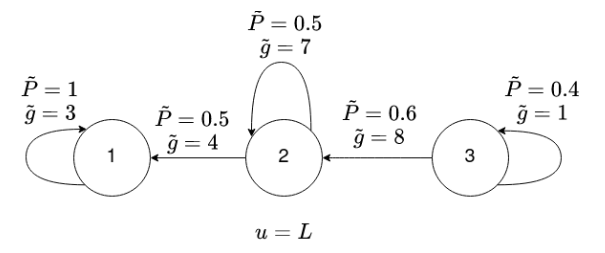
\includegraphics[width=\textwidth]{images/auxSSP_src.png}

\end{minipage}
\hfill
\begin{minipage}{0.475\textwidth}
\centering
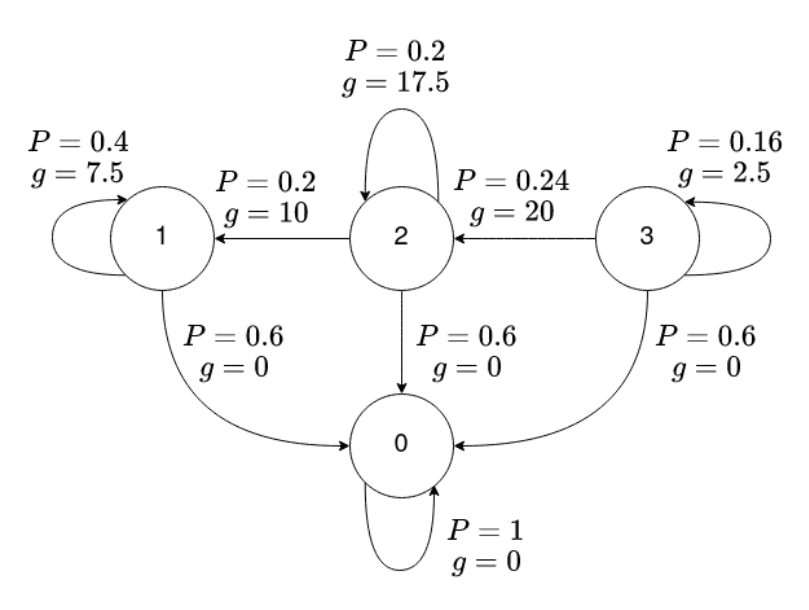
\includegraphics[width=\textwidth]{images/auxSSP_dst.png}
\end{minipage}

}


%----------------------------------------------------------------
%	[SP]Shortest Path
%----------------------------------------------------------------

\headerbox{[SP]Shortest Path}{name=method,column=1,span=2}{
\colorbox[HTML]{CCFFFF}{\makebox[\textwidth-2\fboxsep][l]{\bf [DFS] Deterministic Finite State Problem : }}\vspace{-0.3cm}
$$
x_{k+1} = f_k(x_k,u_k) \\
J = g_N(x_N) + \sum_{k=0}^{N-1}g_k(x_k,u_k)
$$
\colorbox[HTML]{CCFFFF}{\makebox[\textwidth-2\fboxsep][l]{\bf [SP] Shortest Path : }}
In a graph, find a path from node \( s \in \mathcal{V} \) to \( t \in \mathcal{V} \) that has the smallest length:\vspace{-0.4cm}
$$
Q^* = \underset{Q \in \mathbb{Q}_{s,t}}{\text{argmin}} \sum_{h=1}^{q-1}c_{i_h,i_{h+1}}
$$
\begin{minipage}{0.4\textwidth}
\textbf{DFS to SP}
\centering
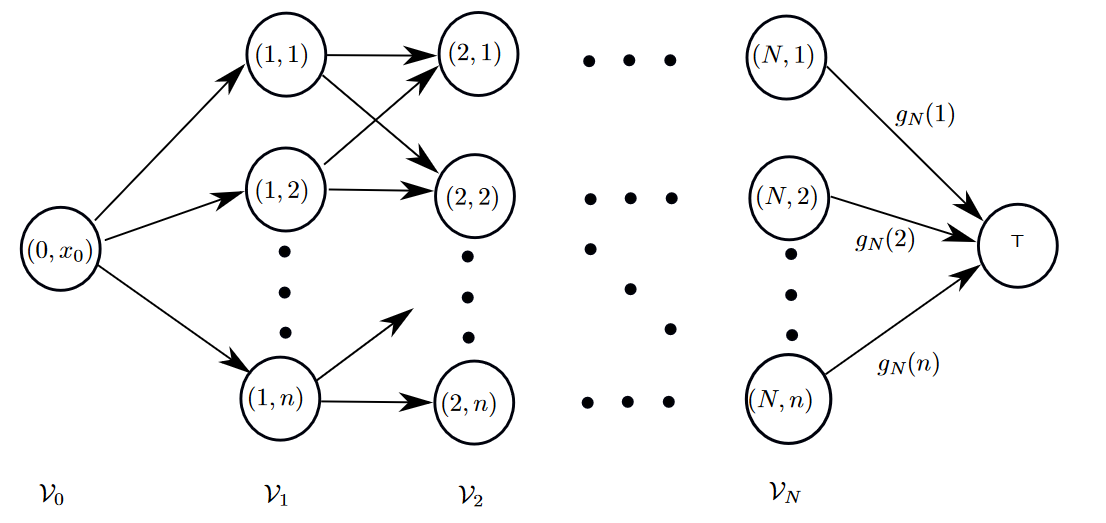
\includegraphics[width=\textwidth]{images/DFS2SP.png}
\end{minipage}
\hfill
\begin{minipage}{0.575\textwidth}
    \begin{itemize}\compresslist
    \item Symmetric: forward DPA and backward DPA are the same for this problem.
      \item No negative cycles: \(\forall i \in \mathcal{V}, Q \in \mathcal{Q}_{i,i}, J_Q \ge 0\). If negative, there will exist an infinite loop.
      \item \( N \le |\mathcal{V}| - 1 \).
        
    \item Why it can be solved by forward DPA (\( J_k \gets J_{k+1} \))? 
    
    It's deterministic.
  \item Why it can be solved by backward DPA (\( J_k \gets J_{k-1} \))? 
  
    It can be converted to a deterministic DP problem.

    \end{itemize}
  
\end{minipage}



  

\colorbox[HTML]{CCFFFF}{\makebox[\textwidth-2\fboxsep][l]{\bf [HMM] Hidden Markov Model : }}
Measurement model: \( z \) is measured in the transition from \( i \) to \( j \):\vspace{-0.3cm}
$$
M_{ij}(z) = p_{z|x,w}(z|i,j)
$$
\colorbox[HTML]{CCFFFF}{\makebox[\textwidth-2\fboxsep][l]{\bf Viterbi Algorithm : }}
Given measured sequence \( Z_1 = (z_1, \cdots, z_N) \), we want to find the most likely state trajectory \( X_0 = (x_0, \cdots, x_N) \):\vspace{-0.5cm}
$$
\begin{aligned}
\underset{X_0}{\text{max}}~p(X_0, Z_1) = p(x_0) \prod_{k=1}^N P_{x_{k-1}x_k}M_{x_{k-1}x_k}(z_k) \Leftrightarrow \underset{X_0}{\text{min}}\left(c_{s,(0,x_0)}+\sum_{k=1}^Nc_{(k-1,x_{k-1}),(k,x_k)}\right)
\end{aligned}
$$
$$
\begin{aligned}
c_{s,(0,x_0)} &= \begin{cases}
-\ln(p(x_0)) & p(x_0) > 0 \\
\infty & p(x_0) = 0
\end{cases} & c_{(N-1,x_{N-1})} = 0
\\
c_{(k-1,x_{k-1}),(k,x_k)} &= \begin{cases}
-\ln(P_{x_{k-1}x_k}M_{x_{k-1}x_k}(z_k)) & P_{x_{k-1}x_k}M_{x_{k-1}x_k}(z_k) > 0 \\
\infty & P_{x_{k-1}x_k}M_{x_{k-1}x_k}(z_k) = 0
\end{cases} 
\end{aligned}
$$

\begin{itemize}\compresslist
  \item DPA can be applied to already solve for the most likely state trajectory up until now.
  \item Future measurements can change the most likely trajectory for past time steps.
\end{itemize}

\colorbox[HTML]{CCFFFF}{\makebox[\textwidth-2\fboxsep][l]{\bf [LCA] Label Correcting Algorithm : }}

\begin{minipage}{0.55\textwidth}\compresslist
    \begin{enumerate}
    \item \(s \to \text{OPEN}\), set \(d_s = 0\), \(d_j = \infty \ \forall j \in \mathcal{V} \setminus \{s\}\).
    \item \(\text{OPEN} \rightarrow \{i\} \cup \text{OPEN}\).
    \item  \(\forall j \in \mathcal{N}_i\) if \((d_i + c_{ij}) < d_j\) and \(\begin{cases}(d_i + c_{ij}) < d_{t}\\(d_i+c_{ij}+h_j)<d_t\end{cases}\)
    \begin{enumerate}
        \item \(d_j \gets d_i + c_{i,j}\)
        \item \(j.\text{parent} \gets i\)
        \item if \(j \neq t\), \(\text{OPEN} \gets \text{OPEN} \cup \{j\}\)
    \end{enumerate}
    \item \(|\text{OPEN}| > 0\) go to 2.
\end{enumerate}
\end{minipage}
\hfill
\begin{minipage}{0.425\textwidth}
    \begin{itemize}
  \item Search Order:
    \begin{itemize}[label=$\circ$]
      \item Breadth-first.
      \item Depth-first.
      \item Best-first: \(d_i\) the smallest nearest first.
    \end{itemize}
  \item\textit{Dijkstra's Algorithm}: \(d_i\) best-first.
  \item \textit{A* Algorithm}: \(d_i +c_{ij} +h_i\) best-first, where \(h_i = \min_{k \in \mathcal{V} \setminus \{j\}} c_{jk}\).
\end{itemize}
\end{minipage}



}


% ----------------------------------------------------------------
% 	[HJB] Hamilton-Jacobian-Bellman Equation
% ----------------------------------------------------------------

\headerbox{[HJB] Hamilton-Jacobian-Bellman}{name=method,column=3}{
\textbf{[HJB] Hamilton-Jacobian-Bellman}

$$
0 = \underset{u \in \mathcal{U}}{\text{min}} \left(g(x,u) + \frac{\partial J^*(t,x)}{\partial t} + \frac{\partial J^*(t,x)}{\partial x} f(x,u)\right)
$$

where \( J^*(T,x) = h(x) \).

\colorbox[HTML]{CCFFFF}{\makebox[\textwidth-2\fboxsep][l]{\bf Pontryagin's Minimum Principle : }}

$$
\begin{aligned}
H(x, u, p) &= g(x, u) + p^\top f(x,u) \\
% \dot{p}(t) &= -\left.\frac{\partial H(x, u, p)}{\partial x}\right|^\top_{\begin{matrix}x(t)\\u(t)\\p(t)\end{matrix}} \\
\dot{p}(t) &= -\left.\frac{\partial H(x, u, p)}{\partial x}\right|_{x = x(t), u = u(t), p = p(t)}^\top\\
p(T) &= \left.\frac{\partial h(x)}{\partial x}\right|^\top_{x(T)} \\
u(t) &= \underset{u \in \mathcal{U}}{\text{argmin}} H(x(t), u, p(t)) \\
\dot{x}(t) &= f(x(t), u(t))
\end{aligned}
$$

\begin{itemize}
  \item Necessary condition for optimal cost.
  \item \textit{Bang-Bang Control}: \( u \in \{a, b\} \)
    \begin{itemize}[label=$\circ$]
      \item Example: \( \ddot{x} = u, a < 0 < b \), 
      
      normally \( u = \begin{cases}b & t \in [0, t] \\ a & t \in [t, T]\end{cases} \)
    \end{itemize}
  \item Minimize total time \( T \): 
  
  \( g(x, u) = 1 \), since \( T = \int_0^T 1 \, d\tau \).
\end{itemize}




\textbf {Optimal Trajectory}
\[
H(x(t), u(t), p(t)) = -\left.\frac{\partial J(t, x)}{\partial t}\right|_{x(t)} = \text{constant}
\]



}

\end{poster}

\end{document}